% This figure was based on a figure of Izaak Neutelings (September 2020)
\documentclass[border=3pt,tikz]{standalone}
\usepackage{amsmath}
\usepackage{tikz}
\usepackage{physics}
\usepackage[outline]{contour} % glow around text
\usetikzlibrary{calc}
\usetikzlibrary{decorations.markings}
\usetikzlibrary{angles,quotes} % for pic
\usetikzlibrary{arrows.meta} % for arrow size
\usetikzlibrary{bending} % for arrow head angle
\usetikzlibrary{decorations.pathmorphing} % for decorate random steps
\tikzset{>=latex} % for LaTeX arrow head
\usepackage{xcolor}
\contourlength{1.3pt}

\colorlet{xcol}{blue!70!black}
\colorlet{xcol'}{xcol!50!red}
\colorlet{vcol}{green!45!black}
\colorlet{acol}{red!50!blue!80!black!80}
\tikzstyle{rvec}=[->,very thick,xcol,line cap=round]
\tikzstyle{vvec}=[->,very thick,vcol,line cap=round]
\tikzstyle{avec}=[->,very thick,acol,line cap=round]
\colorlet{myred}{red!65!black}
\tikzstyle{force}=[->,myred,very thick,line cap=round]
\tikzstyle{mass}=[line width=0.5,draw=red!50!black,fill=red!50!black!10,rounded corners=1,
                  top color=red!50!black!30,bottom color=red!50!black!10,shading angle=20]
\tikzstyle{disk}=[line width=0.5,orange!30!black,fill=orange!40!black!10,
                  top color=orange!40!black!20,bottom color=orange!40!black!10,shading angle=20]
\tikzstyle{pole}=[line width=0.5,blue!20!black,fill=orange!20!black!10,
                  top color=blue!20!black!20,bottom color=blue!20!black!10,shading angle=20]
\tikzstyle{rope}=[brown!70!black,line width=1,line cap=round] %very thick
\tikzstyle{myarr}=[-{Latex[length=3,width=2,flex'=1]},thin]
\tikzstyle{mydashed}=[dash pattern=on 2pt off 1pt]
\def\rope#1{ \draw[rope,black,line width=1.4] #1; \draw[rope,line width=1.1] #1; }
\def\tick#1#2{\draw[thick] (#1) ++ (#2:0.1) --++ (#2-180:0.2)}
\newcommand\rightAngle[4]{
  \pgfmathanglebetweenpoints{\pgfpointanchor{#2}{center}}{\pgfpointanchor{#3}{center}}
  \coordinate (tmpRA) at ($(#2)+(\pgfmathresult+45:#4)$);
  %\draw[white,line width=0.6] ($(#2)!(tmpRA)!(#1)$) -- (tmpRA) -- ($(#2)!(tmpRA)!(#3)$);
  \draw[black] ($(#2)!(tmpRA)!(#1)$) -- (tmpRA) -- ($(#2)!(tmpRA)!(#3)$);
}


\begin{document}

% EARTH + CENTRIFUGAL
\contourlength{0.7pt}
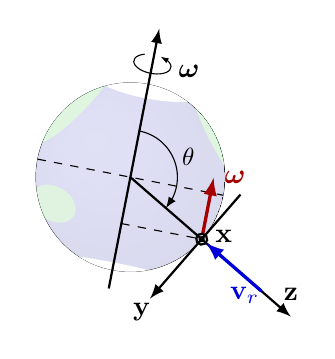
\begin{tikzpicture}
  \def\E{1.2}
  \def\ang{-30} % latidude
  \coordinate (O) at (0,0);
  
  % EARTH
  %\draw[dashed,rotate=-11] (0,-1.3*\E) -- (0,1.45*\E);
  \fill[blue!70!black!70] (0,0) circle (1.2);
  \draw[very thin,ball color=blue!70!black!40,fill opacity=0.2] (0,0) circle (\E);
  \begin{scope}[rotate=-11]
    \draw[-{Latex[length=3,width=2,flex'=1]}]
      (0,1.22*\E)++(120:{0.2*\E} and 0.1*\E) arc(120:430:{0.2*\E} and 0.1*\E)
      node[pos=0.7,right=0] {$\vb*{\omega}$};
    \clip (0,0) circle (\E);
    \fill[white] (0,\E) ellipse ({0.6*\E} and {0.15*\E});
    \fill[white] (0,-\E) ellipse ({0.8*\E} and {0.08*\E});
    \fill[green!70!black!60,rotate=-30] (160:1.1*\E) ellipse ({0.2*\E} and {0.8*\E});
    \fill[green!70!black!60,rotate=40] (-10:1.14*\E) ellipse ({0.2*\E} and {0.9*\E});
    \fill[green!60!black!60,very thick,rotate=-20] % Australia
      (230:0.86*\E) ellipse ({0.25*\E} and {0.18*\E});
    \fill[fill=white,fill opacity=0.8] (0,0) circle (\E);
  \end{scope}
  \begin{scope}[rotate=-11]
    %\draw[dashed] (-\E,0) to[out=-20,in=-160] (\E,0);
    %\draw[->,thick] (-1.2*\E,0) -- (1.2*\E,0);
    \draw[dashed] (-\E,0) -- (\E,0) coordinate (X);
    \draw[dashed] ($(O)+(0,{\E*sin(\ang)})$) -- (\ang:\E) coordinate (R);
 -- (\ang:\E) coordinate (R);
    \draw[->,thick] (0,-1.2*\E) -- (0,1.6*\E);% the omega axis
    \draw[->, thick] (O) -- ($(R)+(\ang:1.5)$) node[pos=1,above=2] {$\vb{z}$};
    \draw[->, thick] ($(R)+(90+\ang:0.75)$) -- ($(R)+(\ang-90:1)$) node[xshift=-3pt, yshift=-5pt] {$\vb{y}$};
    \draw[force] ($(R)+(0,0.075)$) --++ (0,0.6*\E) node[right] {$\vb*{\omega}$};
    \draw[force, blue!85!black] ($(R)+(\ang:1)$) -- ($(R)+(\ang:0.075)$) node[pos=0.3, below] {$\vb{v}_r$};

    % small green circle with an x at R
    \colorlet{gcol}{green!0!black}

    \draw[gcol,thick] (R) circle (0.07);
    \fill[gcol] (R) circle (0.04)
    node[xshift=8pt, yshift=1pt, gcol] {$\vb{x}$};


    % angle theta from rotation axis downward
    \coordinate (A) at ($(90:\E)$);

    \draw pic[<-,"$\theta$"{scale=0.9},
          draw,angle radius=17,angle eccentricity=1.3]
          {angle=R--O--A};


  \end{scope}
  
\end{tikzpicture}


\end{document}